\subsection{Mission d'AMO~: Présentation de \mo}

\begin{frame}
	\frametitle {Mission d'AMO~:Présentation de \mo} 
	\begin{block}{Présentation générale} \pause
	\begin{itemize}
	\item L'une des plus grandes organisations humanitaires au monde \pause
	\item Agit avant, pendant et après les catastrophes et les urgences relatives à la santé \pause
	\item Puise sa force de son réseau de volontaires
	\end{itemize}
	\end{block}
\end{frame}

 %% Présentation de Gk et de son projet.
% Gestion de la planification, du suivi, documentaire.
\begin{frame}
\frametitle {Mission d'AMO~:Présentation de \mo} \pause
   
     \begin{figure}[htbp]
	\centering
	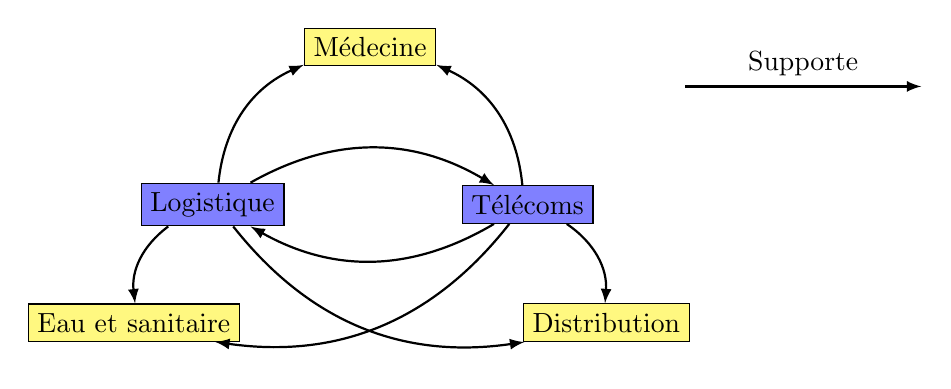
\begin{tikzpicture}
		% définition des styles
		\tikzstyle{metier}=[rectangle,draw,fill=yellow!50,text=black]
		\tikzstyle{support}=[rectangle,draw,fill=blue!50,text=black]
		\tikzstyle{supporte}=[->,>=latex,thick,rounded corners=4pt]
		% les nœuds
		\node[metier] (e) at (-3,-3) {Eau et sanitaire};
		\node[metier] (m) at (0,0.5) {Médecine};
		\node[metier] (d) at (3,-3) {Distribution};
		\node[support] (l) at (-2,-1.5) {Logistique};
		\node[support] (t) at (2,-1.5) {Télécoms};
		% les flèches
		\draw[supporte] (l) to[bend left] (t);
		\draw[supporte] (l) to[bend right] (e);
		\draw[supporte] (l) to[bend left] (m);
		\draw[supporte] (l) to[bend right] (d);
		\draw[supporte] (t) to[bend left] (l);
		\draw[supporte] (t) to[bend left] (e);
		\draw[supporte] (t) to[bend right] (m);
		\draw[supporte] (t) to[bend left] (d);
		% la légende
		\draw[supporte] (4,0) -- (7,0) node[midway,above]{Supporte};
	\end{tikzpicture}
	\caption{Dépendances entre les métiers}
\end{figure}
   
\end{frame}

\begin{frame}
\frametitle {Mission d'AMO~:Présentation de \mo} \pause
\begin{block}{Processus de la logistique} \pause
\begin{enumerate}
\item Achat \pause
\item Stockage \pause
\item Transport
\end{enumerate}
\end{block}

\begin{block}{Fonctions clefs de la logistique} \pause
\begin{enumerate}
\item Planification/évaluation \pause
\item Acquisition/achat \pause
\item Gestion des entrepôts \pause
\item Organisations des transports \pause
\item Suivi et compte rendu
\end{enumerate}
\end{block}

\end{frame}

\begin{frame}
\frametitle {Mission d'AMO~:Présentation de \mo} \pause
\begin{block}{Objectifs de la mission d'AMO pour \mo}
\begin{itemize}
\item Améliorer la qualité de ses services en se dotant d'une solution de type Transport Management System(TMS) 
\item Espérance de retour sur investissement
\end{itemize}
\end{frame}

